% $Author: oscar $
% $Date: 2013-11-27 16:48:27 +0100 (Wed, 27 Nov 2013) $
% $Revision: 35492 $
%=================================================================
\ifx\wholebook\relax\else
% --------------------------------------------
% Lulu:
	\documentclass[a4paper,10pt,twoside]{book}
	\usepackage[
		papersize={6.13in,9.21in},
		hmargin={.815in,.815in},
		vmargin={.98in,.98in},
		ignoreheadfoot
	]{geometry}
	% $Author: oscar $
% $Date: 2009-09-13 20:58:29 +0200 (Sun, 13 Sep 2009) $
% $Revision: 29070 $
%=============================================================
% NB: documentclass must be set in main document.
% Allows book to be generated in multiple formats.
%=============================================================
%:Packages
\usepackage[T1]{fontenc}  %%%%%really important to get the code directly in the text!
\usepackage{palatino}
\usepackage{ifthen}
\usepackage{graphicx}
\graphicspath{{figures/}}
\usepackage{xspace}
\usepackage{makeidx}
\usepackage{isodateo} % enable \isodate
\usepackage{amssymb,textcomp}
%=============================================================
%:More packages
%\usepackage[english]{babel}
%\usepackage{lmodern}
%\usepackage[scaled=0.85]{helvet}
%\usepackage{microtype}
%\usepackage{theorem}
%\usepackage{float}
%\usepackage{longtable}
%\usepackage[nottoc]{tocbibind}
%\usepackage{multicol}
%\usepackage{booktabs}	% book-style tables
%\usepackage{topcapt}	% enables \topcaption
%\usepackage{multirow}
%\usepackage{tabularx}
%\usepackage{alltt}
\usepackage[usenames,dvipsnames]{color}
%\usepackage[hang]{subfigure}\makeatletter\def\p@subfigure{\thefigure\,}\makeatother
%\usepackage{rotating}
%\usepackage{enumitem}	% apb: allows more control over tags in enumerations
%\usepackage{verbatim}     % for comment environment
%\usepackage{varioref}	% for page references that work
%\usepackage{needspace}
%\usepackage[newparttoc]{titlesec}
%\usepackage{titletoc}
%\usepackage{wrapfig}
\usepackage[
	colorlinks=true,
	linkcolor=black,
	urlcolor=black,
	citecolor=black
]{hyperref}   % should come last
%=============================================================
%:URL style
\makeatletter
\def\url@leostyle{%
  \@ifundefined{selectfont}{\def\UrlFont{\sf}}{\def\UrlFont{\sffamily}}}
\makeatother
\urlstyle{leo}
%=============================================================
%:Booleans
\newboolean{lulu}
\setboolean{lulu}{false}
\newcommand{\ifluluelse}[2]{\ifthenelse{\boolean{lulu}}{#1}{#2}}
%=============================================================
%:Editorial comment macros
\newcommand{\nnbb}[2]{
  \fbox{\bfseries\sffamily\scriptsize#1}
  {\sf\small$\blacktriangleright$\textit{#2}$\blacktriangleleft$}
}
\newcommand{\on}[1]{\nnbb{Oscar}{#1}}
\newcommand{\here}{\nnbb{CONTINUE}{HERE}}
%=============================================================
%:Abbreviation macros
\newcommand{\ie}{\emph{i.e.},\xspace}
\newcommand{\eg}{\emph{e.g.},\xspace}
\newcommand{\etc}{\emph{etc.}\xspace}
\newcommand{\etal}{\emph{et al.}\xspace}
\newcommand{\straightquote}{"}
\newcommand{\sba}{\url{SquareBracketAssociates.org}\xspace}
%=============================================================
%:Patterns
% \newcommand{\pattern}[2]{\newpage\section{{\sf #1}}\label{pat:#2}}
% \newcommand{\pattern}[2]{\newpage\index{#1 (Pattern)}\section{#1}\label{pat:#2}}
\newcommand{\pattern}[2]{\cleardoublepage\index{#1 (Pattern)}\section{#1}\label{pat:#2}}
\newcommand{\thumbnail}[2]{\index{#1 (Pattern)}\subsection{#1}\label{pat:#2}}
\newcommand{\thumblang}[2]{\index{#1 (Pattern language)}\subsection{#1}\label{pat:#2}}
\newcommand{\variant}[1]{{\emph{#1}}\xspace}
% \newcommand{\problem}[1]{\subsection*{Problem}\emph{#1}}
\newcommand{\intent}[1]{\paragraph{Intent}\emph{#1}}
\newcommand{\problem}[1]{\paragraph{Problem}\emph{#1}}
\newcommand{\solution}[1]{\paragraph{Solution}\emph{#1}}
\newcommand{\discussion}[0]{\paragraph{Discussion}}
\newcommand{\cmd}[1]{{\tt #1}\xspace}
%=============================================================
%:Environments
\newenvironment{bulletlist}{\begin{itemize}\setlength{\itemsep}{0ex}}
{\end{itemize}}
%=============================================================
%:Cross reference macros
\newcommand{\chalabel}[1]{\label{cha:#1}}
\newcommand{\seclabel}[1]{\label{sec:#1}}
\newcommand{\figlabel}[1]{\label{fig:#1}}
\newcommand{\tablabel}[1]{\label{tab:#1}}
\newcommand{\rulelabel}[1]{\label{rule:#1}}
\newcommand{\eglabel}[1]{\label{eg:#1}}
\newcommand{\scrlabel}[1]{\label{scr:#1}}
\newcommand{\mthlabel}[1]{\label{mth:#1}}
\newcommand{\clslabel}[1]{\label{cls:#1}}
\newcommand{\faqlabel}[1]{\label{faq:#1}}
%\newcommand{\charef}[1]{Chapter~\ref{cha:#1}\xspace}
%\newcommand{\secref}[1]{Section~\ref{sec:#1}\xspace}
\newcommand{\figref}[1]{Figure~\ref{fig:#1}\xspace}
% \newcommand{\patpgref}[2]{\hyperref[pat:#2]{\sf #1} [p.~\pageref{pat:#2}]\xspace}
\newcommand{\patpgref}[2]{\index{#1 (Pattern)}\hyperref[pat:#2]{#1} [p.~\pageref{pat:#2}]\xspace}
\newcommand{\patlangpgref}[2]{\index{#1 (Pattern language)}\hyperref[pat:#2]{#1} [p.~\pageref{pat:#2}]\xspace}
% \newcommand{\patref}[2]{\hyperref[pat:#2]{\sf #1}\xspace}
\newcommand{\patref}[2]{\index{#1 (Pattern)}\hyperref[pat:#2]{#1}\xspace}
\newcommand{\patlangref}[2]{\index{#1 (Pattern language)}\hyperref[pat:#2]{#1}\xspace}
% \newcommand{\charef}[2]{\hyperref[cha:#2]{\underline{\sf #1}}\xspace}
% \newcommand{\charef}[2]{\hyperref[cha:#2]{\sf #1}\xspace}
\newcommand{\charef}[2]{\index{#1 (Pattern cluster)}\hyperref[cha:#2]{#1}\xspace}
% \newcommand{\chapgref}[2]{\hyperref[cha:#2]{\sf #1} [p.~\pageref{cha:#2}]\xspace}
\newcommand{\chapgref}[2]{\index{#1 (Pattern cluster)}\hyperref[cha:#2]{#1} [p.~\pageref{cha:#2}]\xspace}
%\newcommand{\Figref}[1]{Figure~\ref{fig:#1}\xspace}
%\newcommand{\appref}[1]{Appendix~\ref{app:#1}\xspace}
%\newcommand{\tabref}[1]{Table~\ref{tab:#1}\xspace}
%\newcommand{\ruleref}[1]{\ref{rule:#1}\xspace}
%\newcommand{\egref}[1]{example~\ref{eg:#1}\xspace}
%\newcommand{\Egref}[1]{Example~\ref{eg:#1}\xspace}
%\newcommand{\scrref}[1]{script~\ref{scr:#1}\xspace}
%\newcommand{\Scrref}[1]{Script~\ref{scr:#1}\xspace}
%\newcommand{\tscrref}[1]{the script~\ref{scr:#1}\xspace}
%\newcommand{\Tscrref}[1]{The script~\ref{scr:#1}\xspace}
%\newcommand{\mthref}[1]{method~\ref{mth:#1}\xspace}
%\newcommand{\mthsref}[1]{methods~\ref{mth:#1}\xspace}
%\newcommand{\Mthref}[1]{Method~\ref{mth:#1}\xspace}
%\newcommand{\tmthref}[1]{the method~\ref{mth:#1}\xspace}
%\newcommand{\Tmthref}[1]{The method~\ref{mth:#1}\xspace}
%\newcommand{\clsref}[1]{class~\ref{cls:#1}\xspace}
%\newcommand{\tclsref}[1]{the class~\ref{cls:#1}\xspace}
%\newcommand{\Tclsref}[1]{The class~\ref{cls:#1}\xspace}
%=============================================================
%:Page Layout
\setlength{\headsep}{1cm}
%=============================================================
%:Menu item macro
%\definecolor{lightgray}{gray}{0.89}
%\newcommand{\menu}[1]{{%
%	\setlength{\fboxsep}{0pt}%
%	\colorbox{lightgray}{{{\upshape\sffamily\strut \,#1\,}}}}}
%\newcommand{\go}{\,$\triangleright$\,}
%\newcommand{\short}[1]{\mbox{{\sc cmd}\hspace{0.08em}--\hspace{0.09em}#1}\xspace}
%\newcommand{\button}[1]{{%
%	\setlength{\fboxsep}{0pt}%
%	\fbox{{\upshape\sffamily\strut \,#1\,}}}}
%\newcommand{\toolsflap}{\textit{Tools} flap\xspace}
%=============================================================
%:Section depth
%\setcounter{secnumdepth}{2}
%
%\DeclareGraphicsExtensions{.pdf, .jpg, .png}
%=============================================================
%:PDF setup
\hypersetup{
   pdftitle={Object-Oriented Reengineering Patterns},
   pdfauthor={Serge Demeyer, St\'ephane Ducasse, Oscar Nierstrasz},
   pdfkeywords={Reengineering, Object-Oriented Programming, Patterns},
   pdfsubject={Computer Science}
}
%=============================================================
%:Page layout and appearance
%\renewcommand{\chaptermark}[1]{\markboth{#1}{}}
%\renewcommand{\sectionmark}[1]{\markright{\thesection\ #1}}
%\renewpagestyle{plain}[\small\itshape]{%
%	\setheadrule{0pt}%
%	\sethead[][][]{}{}{}%
%	\setfoot[][][]{}{}{}}
%\renewpagestyle{headings}[\small\itshape]{%
%	\setheadrule{0pt}%
%	\setmarks{chapter}{section}%
%	\sethead[\thepage][][\chaptertitle]{\sectiontitle}{}{\thepage}%
%	\setfoot[][][]{}{}{}}
%=============================================================
%:Title section setup and TOC numbering depth
%\setcounter{secnumdepth}{1}
%\setcounter{tocdepth}{1}
%\titleformat{\part}[display]{\centering}{\huge\partname\ \thepart}{1em}{\Huge\textbf}[]
%\titleformat{\chapter}[display]{}{\huge\chaptertitlename\ \thechapter}{1em}{\Huge\raggedright\textbf}[]
%\titlecontents{part}[3pc]{%
%		\pagebreak[2]\addvspace{1em plus.4em minus.2em}%
%		\leavevmode\large\bfseries}
%	{\contentslabel{3pc}}{\hspace*{-3pc}}
%	{}[\nopagebreak]
%\titlecontents{chapter}[3pc]{%
%		\pagebreak[0]\addvspace{1em plus.2em minus.2em}%
%		\leavevmode\bfseries}
%	{\contentslabel{3pc}}{}
%	{\hfill\contentspage}[\nopagebreak]
%\dottedcontents{section}[3pc]{}{3pc}{1pc}
%\dottedcontents{subsection}[3pc]{}{0pc}{1pc}
%\let\origdoublepage\cleardoublepage
%\newcommand{\clearemptydoublepage}{%
%  \clearpage
%  {\pagestyle{empty}\origdoublepage}}
%\let\cleardoublepage\clearemptydoublepage % see http://www.tex.ac.uk/cgi-bin/texfaq2html?label=patch
%=============================================================
%:Listings package configuration
\newcommand{\caret}{\makebox{\raisebox{0.4ex}{\footnotesize{$\wedge$}}}}
% \newcommand{\escape}{{\sf \textbackslash}}
\definecolor{source}{gray}{0.95}
\usepackage{listings}
\lstdefinelanguage{Smalltalk}{
  morestring=[d]',
% Adapt this to other languages!
%  morecomment=[s]{"}{"},
  alsoletter={\#:},
  %escapechar={!},
  literate=
    {BANG}{!}1
%    {UNDERSCORE}{\_}1
    {\\st}{Smalltalk}9 % convenience -- in case \st occurs in code
    % {'}{{\textquotesingle}}1 % replaced by upquote=true in \lstset
%    {_}{{$\leftarrow$}}1
    {>>>}{{\sep}}1
    {^}{{$\uparrow$}}1
    {~}{{$\sim$}}1
    {-}{{\sf -\hspace{-0.13em}-}}1  % the goal is to make - the same width as +
    {+}{\raisebox{0.08ex}{+}}1		% and to raise + off the baseline to match -
    {-->}{{\quad$\longrightarrow$\quad}}3
	, % Don't forget the comma at the end!
  tabsize=4
}[keywords,comments,strings]

\lstset{language=Smalltalk,
	basicstyle=\sffamily,
	keywordstyle=\color{black}\bfseries,
	% stringstyle=\ttfamily, % Ugly! do we really want this? -- on
	mathescape=true,
	showstringspaces=false,
	keepspaces=true,
	breaklines=true,
	breakautoindent=true,
	backgroundcolor=\color{source},
	lineskip={-1pt}, % Ugly hack
	upquote=true, % straight quote; requires textcomp package
	columns=fullflexible} % no fixed width fonts
% \newcommand{\ct}{\lstinline[mathescape=false,basicstyle={\sffamily\upshape}]}
\newcommand{\ct}{\lstinline[mathescape=false,backgroundcolor=\color{white},basicstyle={\sffamily\upshape}]}
\newcommand{\lct}[1]{{\textsf{\textup{#1}}}}
%\newcommand{\scat}[1]{\emph{\textsf{#1}}\xspace}
%\newcommand{\prot}[1]{\emph{\textsf{#1}}\xspace}
% NB: No argument!
\lstnewenvironment{code}[0]{%
	\lstset{%
		% frame=lines,
		frame=single,
		framerule=0pt,
		mathescape=false
	}
}{}
%\def\ignoredollar#1{}
%=============================================================
%:Reserving space
%\newcommand{\needlines}[1]{\Needspace{#1\baselineskip}}
%=============================================================
%:Indexing macros
% Macros ending with "ind" generate text as well as an index entry
% Macros ending with "index" *only* generate an index entry
\newcommand{\ind}[1]{\index{#1}#1\xspace} % plain text
\newcommand{\subind}[2]{\index{#1!#2}#2\xspace} % show #2, subindex under #1
\newcommand{\emphind}[1]{\index{#1}\emph{#1}\xspace} % emph #1
\newcommand{\emphsubind}[2]{\index{#1!#2}\emph{#2}\xspace} % show emph #2, subindex under #1
\newcommand{\patind}[1]{\index{#1@#1 (pattern)}\ct{#1}\xspace} % pattern
\newcommand{\seeindex}[2]{\index{#1|see{#2}}} % #1, see #2
%\newcommand{\boldidx}[1]{{\bf #1}} % breaks hyperlink
%\newcommand{\indmain}[1]{\index{#1}#1\xspace} 
%\newcommand{\emphsubindmain}[2]{\index{#1!#2}\emph{#2}\xspace} % subindex, main entry
%\newcommand{\subindmain}[2]{\index{#1!#2}#2\xspace} % subindex, main entry
%\newcommand{\clsindmain}[1]{\index{#1!\#@(class)}\ct{#1}\xspace} % class main
%\newcommand{\indexmain}[1]{\index{#1}} 
%=============================================================
\parskip 1ex
%=============================================================

	\pagestyle{headings}
	\setboolean{lulu}{true}
% --------------------------------------------
% A4:
%	\documentclass[a4paper,11pt,twoside]{book}
%	% $Author: oscar $
% $Date: 2009-09-13 20:58:29 +0200 (Sun, 13 Sep 2009) $
% $Revision: 29070 $
%=============================================================
% NB: documentclass must be set in main document.
% Allows book to be generated in multiple formats.
%=============================================================
%:Packages
\usepackage[T1]{fontenc}  %%%%%really important to get the code directly in the text!
\usepackage{palatino}
\usepackage{ifthen}
\usepackage{graphicx}
\graphicspath{{figures/}}
\usepackage{xspace}
\usepackage{makeidx}
\usepackage{isodateo} % enable \isodate
\usepackage{amssymb,textcomp}
%=============================================================
%:More packages
%\usepackage[english]{babel}
%\usepackage{lmodern}
%\usepackage[scaled=0.85]{helvet}
%\usepackage{microtype}
%\usepackage{theorem}
%\usepackage{float}
%\usepackage{longtable}
%\usepackage[nottoc]{tocbibind}
%\usepackage{multicol}
%\usepackage{booktabs}	% book-style tables
%\usepackage{topcapt}	% enables \topcaption
%\usepackage{multirow}
%\usepackage{tabularx}
%\usepackage{alltt}
\usepackage[usenames,dvipsnames]{color}
%\usepackage[hang]{subfigure}\makeatletter\def\p@subfigure{\thefigure\,}\makeatother
%\usepackage{rotating}
%\usepackage{enumitem}	% apb: allows more control over tags in enumerations
%\usepackage{verbatim}     % for comment environment
%\usepackage{varioref}	% for page references that work
%\usepackage{needspace}
%\usepackage[newparttoc]{titlesec}
%\usepackage{titletoc}
%\usepackage{wrapfig}
\usepackage[
	colorlinks=true,
	linkcolor=black,
	urlcolor=black,
	citecolor=black
]{hyperref}   % should come last
%=============================================================
%:URL style
\makeatletter
\def\url@leostyle{%
  \@ifundefined{selectfont}{\def\UrlFont{\sf}}{\def\UrlFont{\sffamily}}}
\makeatother
\urlstyle{leo}
%=============================================================
%:Booleans
\newboolean{lulu}
\setboolean{lulu}{false}
\newcommand{\ifluluelse}[2]{\ifthenelse{\boolean{lulu}}{#1}{#2}}
%=============================================================
%:Editorial comment macros
\newcommand{\nnbb}[2]{
  \fbox{\bfseries\sffamily\scriptsize#1}
  {\sf\small$\blacktriangleright$\textit{#2}$\blacktriangleleft$}
}
\newcommand{\on}[1]{\nnbb{Oscar}{#1}}
\newcommand{\here}{\nnbb{CONTINUE}{HERE}}
%=============================================================
%:Abbreviation macros
\newcommand{\ie}{\emph{i.e.},\xspace}
\newcommand{\eg}{\emph{e.g.},\xspace}
\newcommand{\etc}{\emph{etc.}\xspace}
\newcommand{\etal}{\emph{et al.}\xspace}
\newcommand{\straightquote}{"}
\newcommand{\sba}{\url{SquareBracketAssociates.org}\xspace}
%=============================================================
%:Patterns
% \newcommand{\pattern}[2]{\newpage\section{{\sf #1}}\label{pat:#2}}
% \newcommand{\pattern}[2]{\newpage\index{#1 (Pattern)}\section{#1}\label{pat:#2}}
\newcommand{\pattern}[2]{\cleardoublepage\index{#1 (Pattern)}\section{#1}\label{pat:#2}}
\newcommand{\thumbnail}[2]{\index{#1 (Pattern)}\subsection{#1}\label{pat:#2}}
\newcommand{\thumblang}[2]{\index{#1 (Pattern language)}\subsection{#1}\label{pat:#2}}
\newcommand{\variant}[1]{{\emph{#1}}\xspace}
% \newcommand{\problem}[1]{\subsection*{Problem}\emph{#1}}
\newcommand{\intent}[1]{\paragraph{Intent}\emph{#1}}
\newcommand{\problem}[1]{\paragraph{Problem}\emph{#1}}
\newcommand{\solution}[1]{\paragraph{Solution}\emph{#1}}
\newcommand{\discussion}[0]{\paragraph{Discussion}}
\newcommand{\cmd}[1]{{\tt #1}\xspace}
%=============================================================
%:Environments
\newenvironment{bulletlist}{\begin{itemize}\setlength{\itemsep}{0ex}}
{\end{itemize}}
%=============================================================
%:Cross reference macros
\newcommand{\chalabel}[1]{\label{cha:#1}}
\newcommand{\seclabel}[1]{\label{sec:#1}}
\newcommand{\figlabel}[1]{\label{fig:#1}}
\newcommand{\tablabel}[1]{\label{tab:#1}}
\newcommand{\rulelabel}[1]{\label{rule:#1}}
\newcommand{\eglabel}[1]{\label{eg:#1}}
\newcommand{\scrlabel}[1]{\label{scr:#1}}
\newcommand{\mthlabel}[1]{\label{mth:#1}}
\newcommand{\clslabel}[1]{\label{cls:#1}}
\newcommand{\faqlabel}[1]{\label{faq:#1}}
%\newcommand{\charef}[1]{Chapter~\ref{cha:#1}\xspace}
%\newcommand{\secref}[1]{Section~\ref{sec:#1}\xspace}
\newcommand{\figref}[1]{Figure~\ref{fig:#1}\xspace}
% \newcommand{\patpgref}[2]{\hyperref[pat:#2]{\sf #1} [p.~\pageref{pat:#2}]\xspace}
\newcommand{\patpgref}[2]{\index{#1 (Pattern)}\hyperref[pat:#2]{#1} [p.~\pageref{pat:#2}]\xspace}
\newcommand{\patlangpgref}[2]{\index{#1 (Pattern language)}\hyperref[pat:#2]{#1} [p.~\pageref{pat:#2}]\xspace}
% \newcommand{\patref}[2]{\hyperref[pat:#2]{\sf #1}\xspace}
\newcommand{\patref}[2]{\index{#1 (Pattern)}\hyperref[pat:#2]{#1}\xspace}
\newcommand{\patlangref}[2]{\index{#1 (Pattern language)}\hyperref[pat:#2]{#1}\xspace}
% \newcommand{\charef}[2]{\hyperref[cha:#2]{\underline{\sf #1}}\xspace}
% \newcommand{\charef}[2]{\hyperref[cha:#2]{\sf #1}\xspace}
\newcommand{\charef}[2]{\index{#1 (Pattern cluster)}\hyperref[cha:#2]{#1}\xspace}
% \newcommand{\chapgref}[2]{\hyperref[cha:#2]{\sf #1} [p.~\pageref{cha:#2}]\xspace}
\newcommand{\chapgref}[2]{\index{#1 (Pattern cluster)}\hyperref[cha:#2]{#1} [p.~\pageref{cha:#2}]\xspace}
%\newcommand{\Figref}[1]{Figure~\ref{fig:#1}\xspace}
%\newcommand{\appref}[1]{Appendix~\ref{app:#1}\xspace}
%\newcommand{\tabref}[1]{Table~\ref{tab:#1}\xspace}
%\newcommand{\ruleref}[1]{\ref{rule:#1}\xspace}
%\newcommand{\egref}[1]{example~\ref{eg:#1}\xspace}
%\newcommand{\Egref}[1]{Example~\ref{eg:#1}\xspace}
%\newcommand{\scrref}[1]{script~\ref{scr:#1}\xspace}
%\newcommand{\Scrref}[1]{Script~\ref{scr:#1}\xspace}
%\newcommand{\tscrref}[1]{the script~\ref{scr:#1}\xspace}
%\newcommand{\Tscrref}[1]{The script~\ref{scr:#1}\xspace}
%\newcommand{\mthref}[1]{method~\ref{mth:#1}\xspace}
%\newcommand{\mthsref}[1]{methods~\ref{mth:#1}\xspace}
%\newcommand{\Mthref}[1]{Method~\ref{mth:#1}\xspace}
%\newcommand{\tmthref}[1]{the method~\ref{mth:#1}\xspace}
%\newcommand{\Tmthref}[1]{The method~\ref{mth:#1}\xspace}
%\newcommand{\clsref}[1]{class~\ref{cls:#1}\xspace}
%\newcommand{\tclsref}[1]{the class~\ref{cls:#1}\xspace}
%\newcommand{\Tclsref}[1]{The class~\ref{cls:#1}\xspace}
%=============================================================
%:Page Layout
\setlength{\headsep}{1cm}
%=============================================================
%:Menu item macro
%\definecolor{lightgray}{gray}{0.89}
%\newcommand{\menu}[1]{{%
%	\setlength{\fboxsep}{0pt}%
%	\colorbox{lightgray}{{{\upshape\sffamily\strut \,#1\,}}}}}
%\newcommand{\go}{\,$\triangleright$\,}
%\newcommand{\short}[1]{\mbox{{\sc cmd}\hspace{0.08em}--\hspace{0.09em}#1}\xspace}
%\newcommand{\button}[1]{{%
%	\setlength{\fboxsep}{0pt}%
%	\fbox{{\upshape\sffamily\strut \,#1\,}}}}
%\newcommand{\toolsflap}{\textit{Tools} flap\xspace}
%=============================================================
%:Section depth
%\setcounter{secnumdepth}{2}
%
%\DeclareGraphicsExtensions{.pdf, .jpg, .png}
%=============================================================
%:PDF setup
\hypersetup{
   pdftitle={Object-Oriented Reengineering Patterns},
   pdfauthor={Serge Demeyer, St\'ephane Ducasse, Oscar Nierstrasz},
   pdfkeywords={Reengineering, Object-Oriented Programming, Patterns},
   pdfsubject={Computer Science}
}
%=============================================================
%:Page layout and appearance
%\renewcommand{\chaptermark}[1]{\markboth{#1}{}}
%\renewcommand{\sectionmark}[1]{\markright{\thesection\ #1}}
%\renewpagestyle{plain}[\small\itshape]{%
%	\setheadrule{0pt}%
%	\sethead[][][]{}{}{}%
%	\setfoot[][][]{}{}{}}
%\renewpagestyle{headings}[\small\itshape]{%
%	\setheadrule{0pt}%
%	\setmarks{chapter}{section}%
%	\sethead[\thepage][][\chaptertitle]{\sectiontitle}{}{\thepage}%
%	\setfoot[][][]{}{}{}}
%=============================================================
%:Title section setup and TOC numbering depth
%\setcounter{secnumdepth}{1}
%\setcounter{tocdepth}{1}
%\titleformat{\part}[display]{\centering}{\huge\partname\ \thepart}{1em}{\Huge\textbf}[]
%\titleformat{\chapter}[display]{}{\huge\chaptertitlename\ \thechapter}{1em}{\Huge\raggedright\textbf}[]
%\titlecontents{part}[3pc]{%
%		\pagebreak[2]\addvspace{1em plus.4em minus.2em}%
%		\leavevmode\large\bfseries}
%	{\contentslabel{3pc}}{\hspace*{-3pc}}
%	{}[\nopagebreak]
%\titlecontents{chapter}[3pc]{%
%		\pagebreak[0]\addvspace{1em plus.2em minus.2em}%
%		\leavevmode\bfseries}
%	{\contentslabel{3pc}}{}
%	{\hfill\contentspage}[\nopagebreak]
%\dottedcontents{section}[3pc]{}{3pc}{1pc}
%\dottedcontents{subsection}[3pc]{}{0pc}{1pc}
%\let\origdoublepage\cleardoublepage
%\newcommand{\clearemptydoublepage}{%
%  \clearpage
%  {\pagestyle{empty}\origdoublepage}}
%\let\cleardoublepage\clearemptydoublepage % see http://www.tex.ac.uk/cgi-bin/texfaq2html?label=patch
%=============================================================
%:Listings package configuration
\newcommand{\caret}{\makebox{\raisebox{0.4ex}{\footnotesize{$\wedge$}}}}
% \newcommand{\escape}{{\sf \textbackslash}}
\definecolor{source}{gray}{0.95}
\usepackage{listings}
\lstdefinelanguage{Smalltalk}{
  morestring=[d]',
% Adapt this to other languages!
%  morecomment=[s]{"}{"},
  alsoletter={\#:},
  %escapechar={!},
  literate=
    {BANG}{!}1
%    {UNDERSCORE}{\_}1
    {\\st}{Smalltalk}9 % convenience -- in case \st occurs in code
    % {'}{{\textquotesingle}}1 % replaced by upquote=true in \lstset
%    {_}{{$\leftarrow$}}1
    {>>>}{{\sep}}1
    {^}{{$\uparrow$}}1
    {~}{{$\sim$}}1
    {-}{{\sf -\hspace{-0.13em}-}}1  % the goal is to make - the same width as +
    {+}{\raisebox{0.08ex}{+}}1		% and to raise + off the baseline to match -
    {-->}{{\quad$\longrightarrow$\quad}}3
	, % Don't forget the comma at the end!
  tabsize=4
}[keywords,comments,strings]

\lstset{language=Smalltalk,
	basicstyle=\sffamily,
	keywordstyle=\color{black}\bfseries,
	% stringstyle=\ttfamily, % Ugly! do we really want this? -- on
	mathescape=true,
	showstringspaces=false,
	keepspaces=true,
	breaklines=true,
	breakautoindent=true,
	backgroundcolor=\color{source},
	lineskip={-1pt}, % Ugly hack
	upquote=true, % straight quote; requires textcomp package
	columns=fullflexible} % no fixed width fonts
% \newcommand{\ct}{\lstinline[mathescape=false,basicstyle={\sffamily\upshape}]}
\newcommand{\ct}{\lstinline[mathescape=false,backgroundcolor=\color{white},basicstyle={\sffamily\upshape}]}
\newcommand{\lct}[1]{{\textsf{\textup{#1}}}}
%\newcommand{\scat}[1]{\emph{\textsf{#1}}\xspace}
%\newcommand{\prot}[1]{\emph{\textsf{#1}}\xspace}
% NB: No argument!
\lstnewenvironment{code}[0]{%
	\lstset{%
		% frame=lines,
		frame=single,
		framerule=0pt,
		mathescape=false
	}
}{}
%\def\ignoredollar#1{}
%=============================================================
%:Reserving space
%\newcommand{\needlines}[1]{\Needspace{#1\baselineskip}}
%=============================================================
%:Indexing macros
% Macros ending with "ind" generate text as well as an index entry
% Macros ending with "index" *only* generate an index entry
\newcommand{\ind}[1]{\index{#1}#1\xspace} % plain text
\newcommand{\subind}[2]{\index{#1!#2}#2\xspace} % show #2, subindex under #1
\newcommand{\emphind}[1]{\index{#1}\emph{#1}\xspace} % emph #1
\newcommand{\emphsubind}[2]{\index{#1!#2}\emph{#2}\xspace} % show emph #2, subindex under #1
\newcommand{\patind}[1]{\index{#1@#1 (pattern)}\ct{#1}\xspace} % pattern
\newcommand{\seeindex}[2]{\index{#1|see{#2}}} % #1, see #2
%\newcommand{\boldidx}[1]{{\bf #1}} % breaks hyperlink
%\newcommand{\indmain}[1]{\index{#1}#1\xspace} 
%\newcommand{\emphsubindmain}[2]{\index{#1!#2}\emph{#2}\xspace} % subindex, main entry
%\newcommand{\subindmain}[2]{\index{#1!#2}#2\xspace} % subindex, main entry
%\newcommand{\clsindmain}[1]{\index{#1!\#@(class)}\ct{#1}\xspace} % class main
%\newcommand{\indexmain}[1]{\index{#1}} 
%=============================================================
\parskip 1ex
%=============================================================

%	\usepackage{a4wide}
% --------------------------------------------
	\begin{document}
	\renewcommand{\nnbb}[2]{} % Disable editorial comments
	\sloppy
\fi
%=================================================================
\chapter{Initial Understanding}
\chalabel{InitialUnderstanding}

Your company develops and distributes a medical information system named \emph{proDoc} for 
use by doctors. Now the company has bought a competing software \emph{XDoctor} product that 
provides internet support to perform transactions with various health insurance companies. 
The two products should be merged into a single system.

A first evaluation of \emph{XDoctor} has revealed that a few components should somehow be 
recovered and integrated into yours. Of course, to successfully recover a software 
component, you must understand its inner structure as well as its connections with the rest 
of the system. For instance, your company has promised that customers ``won't lose a single 
byte of data'', hence you must recover the database contents and consequently understand 
the database structure and how the upper layers depend on it. Also, your company has 
promised to continue and even expand the transaction support with health insurance 
companies, hence you must recover the network communication component used to communicate 
with these remote services.

\subsection*{Forces}

Situations similar to this one occur frequently in reengineering projects. After the 
\chapgref{First Contact}{FirstContact} with the system and its users, it is clear what kind 
of functionality is valuable and why it must be recovered. However, you lack knowledge 
about the overall design of the software system, so you cannot predict whether this 
functionality can be lifted out of the legacy system and how much effort that will cost 
you. Such initial understanding is crucial for the success of a reengineering project and 
this chapter will explain how to obtain it.

The patterns in \charef{First Contact}{FirstContact} should have helped you to get some 
first ideas about the software system. Now is the right time to refine those ideas into an 
initial understanding and to document that understanding in order to support further 
reverse engineering activities. The main priority at this stage of reverse engineering is 
to set up a reliable foundation for the rest of your project, thus you must make sure that 
your discoveries are correct and properly documented.

How to properly document your discoveries depends largely on the scope of your project and 
the size of the your team. A complicated reverse engineering project involving more than 
ten developers, demands some standard document templates and a configuration management 
system. At the other extreme, a run-of-the-mill project involving less than three persons 
may be able to manage just fine with some loosely structured files shared on a central 
server. However, there are a few inherent forces that apply to any situation.

\begin{bulletlist}
\item \emph{Data is deceptive.}
To understand an existing software system you must collect and interpret data and summarize 
it in a coherent view. There is usually more than one way to interpret data and when 
choosing between alternatives you will make assumptions that are not always backed up by 
concrete evidence. \emph{Consequently, double-check your sources to make sure you build 
your understanding on a solid foundation.}

\item \emph{Understanding entails iteration.}
Understanding occurs inside the human brain, thus corresponds to a kind of learning 
process. Reverse engineering techniques must support the way our minds assimilate new 
ideas, hence be very flexible and allow for a lot of iteration and backtracking. 
\emph{Consequently, plan for iteration and feedback loops in order to stimulate a learning 
process.}

\item \emph{Knowledge must be shared.}
Once you understand the system it is important to share this knowledge with your 
colleagues. Not only will it help them to do their job, it will also result in comments and 
feedback that may improve your understanding. \emph{Therefore, put the map on the wall:} 
publish your discoveries in a highly visible place and make explicit provisions for 
feedback. How to do this will depend on the team organization and working habits. Team 
meetings in general are a good way to publish information (see \patpgref{Speak to the Round 
Table}{SpeakToTheRoundTable}), but a large drawing on the wall near the coffee machine may 
serve just as well.

\item \emph{Teams need to communicate.}
Building and documenting your understanding of a system is not a goal; it is a means to 
achieve a goal. The real goal of understanding the system is to communicate effectively 
with the other persons involved in the project, thus the way you document your 
understanding must support that goal. There is for instance no point in drawing UML class 
diagrams if your colleagues only know how to read ER-diagrams; there is no point in writing 
use cases if your end users can't understand their scope. \emph{Consequently, use their 
language:} choose the language for documenting your understanding so that your team members 
can read, understand and comment on what you have documented.
\end{bulletlist}

\subsection*{Overview}

When developing your initial understanding of a software system, incorrect information is 
your biggest concern. Therefore these patterns rely mainly on source-code because this is 
the only trustworthy information source.

In principle, there are two approaches for studying source-code: one is top-down, the other 
is bottom-up. In practice, every reverse engineering approach must incorporate a little bit 
of both, still it is worthwhile to make the distinction. With the top-down approach, you 
start from a high-level representation and verify it against the source-code (as for 
instance described in \patref{Speculate about Design}{SpeculateAboutDesign}). In the 
bottom-up approach, you start from the source-code, filter out what's relevant and cast the 
relevant entities into a higher-level representation. This is the approach used in 
\patref{Analyze the Persistent Data}{AnalyzeThePersistentData} and \patref{Study the 
Exceptional Entities}{StudyTheExceptionalEntities}.

There is no preferred order in which to apply each of these patterns. It may be natural to 
first \patref{Analyze the Persistent Data}{AnalyzeThePersistentData}, then refine the 
resulting model via \patref{Speculate about Design}{SpeculateAboutDesign} and finally 
exploit this knowledge to \patref{Study the Exceptional Entities}
{StudyTheExceptionalEntities}. Therefore the patterns are presented in that order. However, 
large parts of your system won't have anything to do with a database (some systems lack any 
form of persistent data) and then \patref{Speculate about Design}{SpeculateAboutDesign} 
must be done without having studied the database. And when you lack the inspiration to 
start with \patref{Speculate about Design}{SpeculateAboutDesign}, then \patref{Study the 
Exceptional Entities}{StudyTheExceptionalEntities} will surely provide you with an initial 
hypothesis.

\begin{figure}
\begin{center}
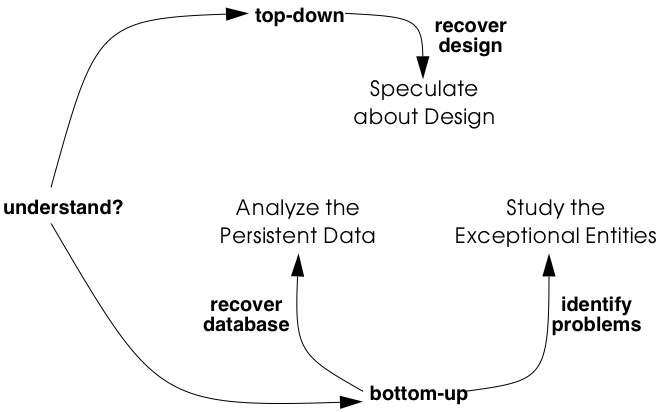
\includegraphics[width=\textwidth]{InitialUnderstandingMap}
\caption{Obtain an \charef{Initial Understanding}{InitialUnderstanding} of a software 
system and cast it into a higher-level representation.}
\figlabel{InitialUnderstandingMap}
\end{center}
\end{figure}

The amount of time you should devote to each of these patterns depends largely on the goal 
of your reengineering project. In principle, none of these patterns will take long, but 
each of them should be applied several times. You cannot predict how many cycles will be 
necessary, because the assessment whether your team understands enough to proceed with the 
rest of the project can only be done after the patterns have been applied. Therefore, these 
patterns must be applied on a case-by-case basis.

\subsection*{What Next}

You should make sure to reflect your increased understanding in the project plan. For 
instance, \patref{Analyze the Persistent Data}{AnalyzeThePersistentData} and 
\patref{Speculate about Design}{SpeculateAboutDesign} will document parts of the system, 
and this documentation must be added to the Opportunities. On the other hand, \patref{Study 
the Exceptional Entities}{StudyTheExceptionalEntities} will reveal some suspicious 
components and these must be added to the Risks.

Once you have obtained a solid foundation for your understanding, you should fill in the 
details for those components that are important for the rest of your project. Activities 
described in \chapgref{Detailed Model Capture}{DetailedModelCapture} may help you to fill 
in those details.

%=================================================================
%:PATTERN -- {Analyze the Persistent Data}
\pattern{Analyze the Persistent Data}{AnalyzeThePersistentData}

\intent{Learn about objects that are so valuable they must be kept inside a database 
system.}

\subsection*{Problem}

Which object structures represent the valuable data ?

\emph{This problem is difficult because:}

\begin{bulletlist}
\item Valuable data must be kept safe on some external storage device (\ie a file system, a 
\ind{database}). However, such data stores often act as an attic: they are rarely cleaned 
up and may contain lots of junk.

\item When loaded in memory, the valuable data is represented by complex object structures. 
Unfortunately there lies a big gap between the data structures provided by external storage 
devices and the object structures living in main memory. Inheritance relationships for 
instance are seldom explicitly provided in a legacy database.

\item ``Valuable'' is a relative property. It is possible that large parts of the saved 
data are irrelevant for your reengineering project.
\end{bulletlist}

\emph{Yet, solving this problem is feasible because:}

\begin{bulletlist}
\item The software system employs some form of a database to make its data persistent. Thus 
there exists some form of database schema providing a static description of the data inside 
the database.

\item The database comes with the necessary tools to inspect the actual objects inside the 
database, so you can exploit the presence of legacy data to fine-tune your findings.

\index{database!schema}
\item You have some expertise with mapping data-structures from your implementation 
language onto a database schema, enough to reconstruct a class diagram from the database 
schema.

\item You have a rough understanding of the system's functionality and the goals of your 
project (for example obtained via \charef{First Contact}{FirstContact}), so you can assess 
which parts of the database are valuable for your project.
\end{bulletlist}

\subsection*{Solution}

Analyze the database schema and filter out which structures represent valuable data. Derive 
a \subind{UML}{class diagram} representing those entities to document that knowledge for 
the rest of the team.

\subsubsection*{Steps}

The steps below assume that the system makes use of a \emph{relational database}, which is 
commonly the case for object-oriented applications. However, in case you're confronted with 
another kind of database system, many of these steps may still be applicable. The steps 
themselves are guidelines only: they must be applied iteratively, with liberal doses of 
intuition and backtracking.

\noindent
\emph{Preparation.}
To derive a class diagram from a relational database schema, first prepare an initial model 
representing the tables as classes. You may do this by means of a software tool, but a set 
of index cards may serve just as well.

\begin{enumerate}
  \item Enumerate all table names and for each one, create a class with the same name.

  \item For each table, collect all column names and add these as attributes to the 
corresponding class.

  \item For each table, determine candidate keys. Some of them may be read directly from 
the database schema, but usually a more detailed analysis is required. Certainly check all 
(unique) indexes as they often suggest candidate keys. Naming conventions (names including 
ID or \#) may also indicate candidate keys. In case of doubt, collect data samples and 
verify whether the candidate key is indeed unique within the database population.

  \item Collect all foreign keys relationships between tables and create an association 
between the corresponding classes. Foreign key relationships may not be maintained 
explicitly in the database schema and then you must infer these from column types and 
naming conventions. Careful analysis is required here, as homonyms (= identical column name 
and type, yet different semantics) and synonyms (= different column name or type, yet 
identical semantics) may exist. To cope with such difficulties, at least verify the indexes 
and view declarations as these point to frequent traversal paths. If possible, verify the 
join clauses in the \ind{SQL} statements executed against the database. Finally, confirm or 
refute certain foreign key relationships by inspecting data samples.

\end{enumerate}

\begin{figure}
\begin{center}
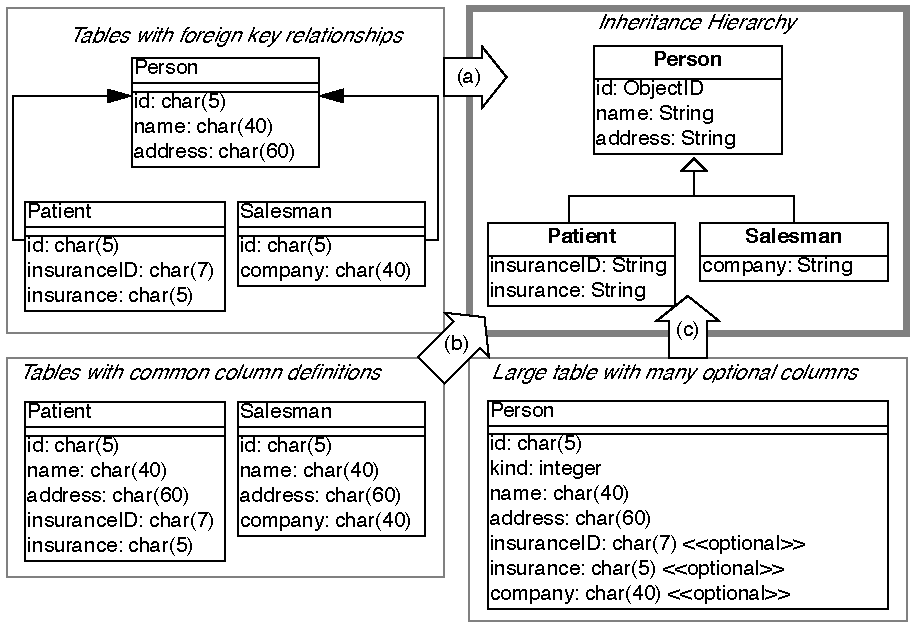
\includegraphics[width=\textwidth]{InitialMappingRelations}
\caption{Mapping a series of relational tables onto an inheritance hierarchy. (a) one to 
one; (b) rolled down; (c) rolled up}
\figlabel{InitialMappingRelations}
\end{center}
\end{figure}

\noindent
\emph{Incorporate inheritance.}
After the above steps, you will have a set of classes that represents the tables being 
stored in the relational database. However, because relational databases cannot represent 
inheritance relationships, you have to infer these from the foreign keys. (The terminology 
for the three representations of inheritance relations in steps 5-7 stems from 
\cite{Fros94a}.)

\begin{enumerate}\setcounter{enumi}{4}
  \item \emph{One to one} (\figref{InitialMappingRelations} (a)). Check tables where the 
primary key also serves as a foreign key to another table, as such foreign keys may 
represent inheritance relationships. Examine the SELECT statements that are executed 
against these tables to see whether they usually involve a join over this foreign key. If 
this is the case, analyze the table names and the corresponding source code to verify 
whether this foreign key indeed represents an inheritance relationship. If it does, 
transform the association that corresponds with the foreign key into an inheritance 
relationship.

  \item \emph{Rolled down} (\figref{InitialMappingRelations} (b)). Check tables with common 
sets of column definitions, as these probably indicate a situation where the class 
hierarchy is spread over several tables, each table representing one non-abstract class. 
Define a common superclass for each cluster of duplicated column definitions and move the 
corresponding attributes inside the new class. Check the source code for the name 
applicable for the newly created classes.

  \item \emph{Rolled up} (\figref{InitialMappingRelations} (c)). Check tables with many 
columns and lots of optional attributes as these may indicate a situation where a complete 
class hierarchy is represented in a single table. If you have found such a table, examine 
all the SELECT statements that are executed against this table. If these SELECT statements 
explicitly request for subsets of the columns, then you may break this one class into 
several classes depending on the subsets requested. For the names of these classes, check 
for an encoding of subtype information like for instance a ``kind'' column holding an 
enumeration type number.

\end{enumerate}

\noindent
\emph{Incorporate associations.}
Note that the class diagram extracted from the database may be too small: it is possible 
that classes in the actual inheritance hierarchy have been omitted in the database because 
they did not define any new attributes. Also, table- and column-names may sound bizarre. 
Therefore, consider to verify the class diagram against the source code (see 
\patref{Speculate about Design}{SpeculateAboutDesign}) as this may provide extra insight. 
Afterwards, refine the remaining associations.

\begin{enumerate}\setcounter{enumi}{7}
  \item Determinate association classes, \ie classes that represent the fact that two 
objects are associated. The most common example is a many-to-many association, which is 
represented by a table having a candidate key consisting of two foreign keys. In general, 
all tables where the candidate keys are concatenations of multiple foreign keys are 
potential cases of an association class.

  \item Merge complementary associations. Sometimes a class A will have a foreign key 
association to class B and class B an inverse foreign key to class A. In that case, merge 
the two associations into a single association navigable in both directions.

  \item Resolve \ind{foreign key} targets. When inheritance hierarchies have been rolled up 
or down in the database, foreign key targets may become ambiguous after the table has been 
decomposed in its constituting classes. Foreign key targets may be too high or too low in 
the hierarchy, in which case the corresponding association will have too little or too many 
participating classes. Resolving such situation typically requires analyzing data-samples 
and \ind{SQL} statements to see which classes actually participate in the association.

  \item Identify qualified associations, \ie associations that can be navigated by 
providing a certain look-up key (the qualifier). Common examples are ordered one-to-many 
associations, where the ordering number serves as the qualifier. In general, all tables 
where the candidate key combines a foreign key with extra columns are potential qualified 
associations; the extra columns then represent the qualifier.

  \item Note multiplicities for the associations. Since all associations are derived from 
foreign key relationships, all associations are by construction optional 1-to-many 
associations. However, by inspecting non-null declarations, indices and data samples one 
can often determine the minimum and maximum multiplicities for each of the roles in the 
association.

\end{enumerate}

\noindent
\emph{Verification.}
Note the recurring remark that the database schema alone is too weak as a basis to derive a 
complete class diagram. Fortunately, a legacy system has a populated database and programs 
manipulating that database. Hence, data samples and embedded \ind{SQL} statements can be 
used to verify the reconstructed classes.

\begin{bulletlist}
\item \emph{Data samples.}
Database schemas only specify the constraints allowed by the underlying database system and 
model. However, the problem domain may involve other constraints not expressed in the 
schema. By inspecting samples of the actual data stored in the database you can infer other 
constraints.

\item \emph{\ind{SQL} statements.}
Tables in a relational database schema are linked via foreign keys. However, it is 
sometimes the case that some tables are always accessed together, even if there is no 
explicit foreign key. Therefore, it is a good idea to check which queries are actually 
executed against the database engine. One way to do this is to extract all embedded 
\ind{SQL} statements in the program. Another way is to analyze all executed queries via the 
tracing facilities provided with the database system.
\end{bulletlist}

\noindent
\emph{Incorporate operations.}
It should be clear that the \subind{UML}{class diagram} you extract from a database will 
only represent the data-structure, not the operations used to manipulate those structures. 
As such, the resulting class diagram is necessarily incomplete. By comparing the code with 
the model extracted from the database (see \patref{Speculate about Design}
{SpeculateAboutDesign} and \patpgref{Look for the Contracts}{LookForTheContracts}) it is 
possible to incorporate the operations for the extracted classes.

\subsection*{Tradeoffs}

\subsubsection*{Pros}

\begin{bulletlist}
\item \emph{Improves team communication.} By capturing the database schema you will improve 
the communication within the reengineering team and with other developers associated with 
the project (in particular the maintenance team). Moreover, many if not all of the people 
associated with the project will be reassured by the fact that the data schema is present, 
because lots of development methodologies stress the importance of the database design.

\item \emph{Focus on valuable data.} A database provides special features for backup and 
security and is therefore the ideal place to store the valuable data. Once you understand 
the database schema it is possible to extract the valuable data and preserve it during 
future reengineering activities.
\end{bulletlist}

\subsubsection*{Cons}

\begin{bulletlist}
\item \emph{Has limited scope.}
Although the database is crucial in many of today's software systems, it involves but a 
fraction of the complete system. As such, you cannot rely on this pattern alone to gain a 
complete view of the system.

\item \emph{Junk data.}
A database will contain a lot more than the valuable data and depending on how old the 
legacy system is a lot of junk data may be stored just because nobody did care to remove 
it. \emph{Therefore, you must match the database schema you recovered against the needs of 
your reengineering project.}

\item \emph{Requires database expertise.}
The pattern requires a good deal of knowledge about the underlying database plus structures 
to map the database schema into the implementation language. As such, the pattern should 
preferably be applied by people having expertise in mappings from the chosen database to 
the implementation language.

\item \emph{Lacks behavior.}
The class diagram you extract from a database is very data-oriented and includes little or 
no behavior. A truly object-oriented class diagram should encapsulate both data and 
behavior, so in that sense the database schema shows only half of the picture. However, 
once the database model exists, it is possible to add the missing behavior later.
\end{bulletlist}

\subsubsection*{Difficulties}

\begin{bulletlist}
\item \emph{Polluted database schema.}
The database schema itself is not always the best source of information to reconstruct a 
class diagram for the valuable objects. Many projects must optimize database access and as 
such often sacrifice a clean database schema. Also, the database schema itself evolves over 
time, and as such will slowly deteriorate. \emph{Therefore, it is quite important to refine 
the class diagram via analysis of data samples and embedded \ind{SQL} statements.}
\end{bulletlist}

\subsection*{Example}

While taking over \emph{XDoctor}, your company has promised to continue to support the 
existing customer base. In particular, you have guaranteed customers that they won't lose a 
single byte of data, and now your boss asks you to recover the database structure. From the 
experience with your own product, you know that doctors care a lot about their patient 
files and that it is unacceptable to lose such information. Therefore you decide that you 
will start by analyzing the way patient files are stored inside the database.

\begin{figure}
\begin{center}
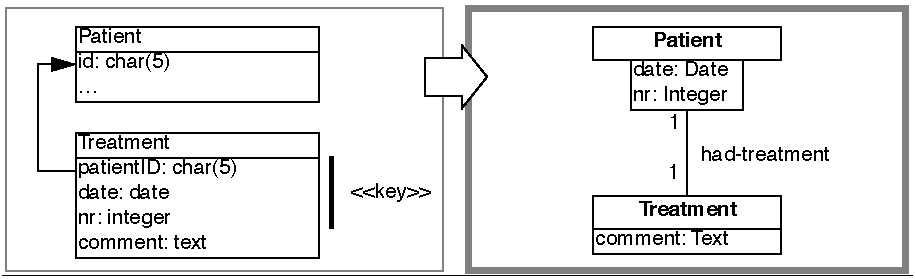
\includegraphics[width=\textwidth]{InitialQualified}
\caption{Identify a qualified association via a key consisting of a foreign key (patientID) 
and two extra columns (date, nr).}
\figlabel{InitialQualified}
\end{center}
\end{figure}

You start by browsing all table names looking for a table named \lct{Patient}, but 
unfortunately you don't find one. However, there is a close match in a table named 
\lct{Person}, where column names like \lct{insuranceID} suggest that at least some patient 
information is stored. Nevertheless, many column names are optional, so you suspect a 
rolled up representation where patient information is mixed with information from other 
kinds of persons. Therefore, you check the source-code and look for all embedded SQL 
statements querying the table \lct{Person} (\ie \lct{grep "SELECT * Person"}). Indeed, 
there are two classes where such a query is used, namely \lct{Patient} and \lct{Salesman} 
and from the subsets of columns queried in each class, you infer the inheritance hierarchy 
depicted in \figref{InitialMappingRelations}.

Now that you recovered the \lct{Patient}, you start looking for the table that stores the 
treatments a patient received. And indeed there is a table \lct{Treatment} which has a 
foreign key to the table \lct{Person}. However, since you have decomposed \lct{Person} into 
the classes \lct{Patient} and \lct{Salesman}, it is necessary to resolve the target of the 
foreign key. You join the tables \lct{Person} and \lct{Treatment} over \lct{patientID 
(SELECT DISTINCT name, kind FROM Person, Treatment WHERE Person.id = Treatment.patientID}) 
and see that all selected persons indeed have a kind which corresponds to a \lct{Patient}. 
Therefore, you set the target of the foreign key leaving from \lct{Treatment} to 
\lct{Patient} (see left side of \figref{InitialMappingRelations}). Next, you verify the 
indices defined on \lct{Treatment} and notice that there is a unique index on the columns 
\lct{patientID - date - nr}, which makes you conclude that these columns serve as a 
candidate key. Since the candidate key on \lct{Treatment} consists of a foreign key 
combined with two extra columns, you suspect a qualified association. To confirm this 
assumption you analyze a data sample (\lct{SELECT name, date, nr FROM Person, Treatment 
WHERE Person.id = Treatment.patientID ORDER BY name, date, nr}) and see that the date and 
the number uniquely identify a treatment for a given patient. As a consequence, you 
transform the foreign key into a qualified association had-treatment with a multiplicity of 
one on each role.

\subsection*{Rationale}

\index{Blaha, Michael}
\begin{quotation}
\noindent
\emph{The object model is important for database applications because it concisely describes data structure and captures structural constraints.}

\hfill --- Michael Blaha, \etal. \cite{Blah98a} 
\end{quotation}

Having a well-defined central database schema is a common practice in larger software 
projects that deal with persistent data. Not only does it specify common rules on how to 
access certain data structures, it is also a great aid in dividing the work between team 
members. Therefore, it is a good idea to extract an accurate model of the database before 
proceeding with other reverse engineering activities.

Note that extracting a database model is essentially a bottom-up approach: you start from 
the rough information contained in the database schema and you polish it up until you have 
a satisfactory class diagram. A bottom up approach works quite well in such a situation, 
because a database schema is already an abstraction from a more detailed representation.

\index{Riel, Arthur}
\begin{quotation}
\noindent
\emph{All data should be hidden within its class.}

\hfill --- Arthur Riel, Heuristic 2.1 \cite{Riel96a}
\end{quotation}

Information hiding is an important design principle, and most authors agree that for a 
class this implies that all data should be encapsulated within the class and only accessed 
via the operations defined on that class. Unfortunately, the class diagram you extract from 
a database will expose all of its data, because that's the nature of a database. Therefore, 
this class diagram is just a first step towards a well-designed interface to the database.

\subsection*{Known Uses}

The reverse engineering and reengineering of database systems is a well-explored area of 
research \cite{Arno92a} \cite{Mull00a}. Several experiments indicate that it is feasible to 
recover the database structure, even for these database systems that are poorly designed. 
\cite{Prem94a} for instance reports about an experiment concerning the reverse engineering 
of a data dictionary of a leading RDBMS vendor, as well as a production database storing 
data about mechanical parts. \cite{Hain96a} describes a prototype database reverse 
engineering toolkit, as well as five industrial cases where the toolkit has been applied. 
To illustrate the unpredictable nature of database reverse engineering, \cite{Jahn97b} 
reports on the use of a fuzzy reasoning engine as the core of a tool that extracts class 
diagrams out of relational database schemas.

\subsection*{What Next}

\patref{Analyze the Persistent Data}{AnalyzeThePersistentData} results in a class diagram 
for the persistent data in your software system. Such a class diagram is quite rough and is 
mainly concerned with the structure of the data and not with its behavior. However, it may 
serve as an ideal initial hypothesis to be further refined by applying \patref{Speculate 
about Design}{SpeculateAboutDesign} and \patpgref{Look for the Contracts}
{LookForTheContracts}.

If you need to migrate to another database, you should cast your understanding of the 
database model in a test suite as explained in \chapgref{Tests: Your Life Insurance!}
{TestsYourLifeInsurance}.

Note that there exist patterns, idioms and pattern languages that describe various ways to 
map object-oriented data structures on relational database counterparts \cite{Brow96d} 
\cite{Kell98a}. Consulting these may help you when you are reverse engineering a database 
schema.

%=================================================================
%:PATTERN -- {Speculate about Design}
\pattern{Speculate about Design}{SpeculateAboutDesign}

\intent{Progressively refine a design against source code by checking hypotheses about the 
design against the source code.}

\subsection*{Problem}

How do you recover the way design concepts are represented in the source-code?

\emph{This problem is difficult because:}

\begin{bulletlist}

\item There are many design concepts and there are countless ways to represent them in the 
programming language used.

\item Much of the source-code won't have anything to do with the design but rather with 
implementation issues (glue code, user-interface control, database connections,-).
\end{bulletlist}

\emph{Yet, solving this problem is feasible because:}

\begin{bulletlist}
\item You have a \emph{rough understanding} of the system's functionality (for example 
obtained via \patpgref{Skim the Documentation}{SkimTheDocumentation} and 
\patpgref{Interview During Demo}{InterviewDuringDemo}), and you therefore have an initial 
idea which design issues should be addressed.

\item You have \emph{development expertise}, so you can imagine how you would design the 
problem yourself.

\item You are \emph{somewhat familiar} with the main structure of the source code (for 
example obtained by \patpgref{Read all the Code in One Hour}{ReadAllTheCodeInOneHour}) so 
that you can find your way around.
\end{bulletlist}

\subsection*{Solution}

Use your development expertise to conceive a hypothetical class diagram representing the 
design. Refine that model by verifying whether the names in the class diagram occur in the 
source code and by adapting the model accordingly. Repeat the process until your class 
diagram stabilizes.

\subsubsection*{Steps}
\begin{enumerate}
  \item With your understanding of the system, develop a class diagram that serves as your 
initial hypothesis of what to expect in the source code. For the names of the classes, 
operations and attributes make a guess based on your experience and potential naming 
conventions (see \patpgref{Skim the Documentation}{SkimTheDocumentation}).

  \item Enumerate the names in the class diagram (that is, names of classes, attributes and 
operations) and try to find them in the source code, using whatever tools you have 
available. Take care as names inside the source-code do not always match with the concepts 
they represent.\footnote{In one particular reverse engineering experience, we were facing 
source code that was a mixture of English and German. As you may expect, this complicates 
matters a lot.} To counter this effect, you may rank the names according to the likelihood 
that they appear in the source code.

  \item Keep track of the names that appear in source code (confirm your hypothesis) and 
the names which do not match with identifiers in the source code (contradict your 
hypothesis). Remember that mismatches are positive, as these will trigger the learning 
process that you must go through when understanding the system.

  \item Adapt the class diagram based on the mismatches. Such adaptation may involve

(a) \emph{renaming}, when you discover that the names chosen in the source code do not 
match with your hypothesis;

(b) \emph{remodelling}, when you find out that the source-code representation of the design 
concept does not correspond with what you have in your model. For instance, you may 
transform an operation into a class, or an attribute into an operation.

(c) \emph{extending}, when you detect important elements in the source-code that do not 
appear in your class diagram;

(d) \emph{seeking alternatives}, when you do not find the design concept in the source-
code. This may entail trying synonyms when there are few mismatches but may also entail 
defining a completely different class diagram when there are lots of mismatches.

  \item Repeat steps 2-4 until you obtain a class diagram that is satisfactory.

\end{enumerate}

\subsubsection*{Variants}

\variant{Speculate about Business Objects.}
A crucial part of the system design is the way concepts of the problem domain are 
represented as classes in the source code. You can use a variant of this pattern to extract 
those so-called ``business objects''.

One way to build an initial hypothesis is to use the noun phrases in the requirements as 
the initial class names and the verb phrases as the initial method names (See 
\cite{Wirf90b} \cite{Bell97a} \cite{Booc94a} for in-depth treatments of finding classes and 
their responsabilities).You should probably augment this information via the usage 
scenarios that you get out of \patpgref{Interview During Demo}{InterviewDuringDemo} which 
may help you to find out which objects fulfil which roles. (See \cite{Jaco92a} 
\cite{Schn98a} for scenarios and use cases and \cite{Reen96a} \cite{Rieh98a} for role 
modeling.)

\variant{Speculate about Patterns.}
Patterns are ``recurring solutions to a common design problem in a given context''. Once 
you know where a certain pattern has been applied, it reveals a lot about the underlying 
system design. This variant verifies a hypothesis about occurrences of architectural 
\cite{Busc96a}, analysis \cite{Fowl97b} or design patterns \cite{Gamm95a}.

\variant{Speculate about Architecture.}
``A software \ind{architecture} is a description of the subsystem and components of a 
software system and the relationships between them'' \cite{Busc96a} (a.k.a. Components and 
Connectors \cite{Shaw96a}). The software architecture is typically associated with the 
coarse level design of a system and as such it is crucial in understanding the overall 
structure. Software architecture is specially relevant in the context of a distributed 
system with multiple cooperating processes, an area where reverse engineering is quite 
difficult.

This variant builds and refines a hypothesis about which components and connectors exist, 
or in the context of a distributed system, which processes exist, how they are launched, 
how they get terminated and how they interact. Consult \cite{Busc96a} for a catalogue of 
architectural patterns and \cite{Shaw96a} for a list of well-known architectural styles. 
See \cite{Lea96a} for some typical patterns and idioms that may be applied in concurrent 
programming and \cite{Schm00a} for architectural patterns in distributed systems.

\subsection*{Tradeoffs}

\subsubsection*{Pros}

\begin{bulletlist}
\item \emph{Scales well.}
Speculating about what you'll find in the source code is a technique that scales up well. 
This is especially important because for large object-oriented programs (over a 100 
classes) a bottom-up approach quickly becomes impractical.

\item \emph{Investment pays off.}
The technique is quite cheap in terms of resources and tools, definitely when considering 
the amount of understanding one obtains.
\end{bulletlist}

\subsubsection*{Cons}

\begin{bulletlist}
\item \emph{Requires expertise.}
A large repertoire of knowledge about idioms, patterns, algorithms, techniques is necessary 
to recognize what you see in the source code. As such, the pattern should preferably be 
applied by experts.

\item \emph{Consumes much time.}
Although the technique is quite cheap in terms of resources and tools, it requires a 
substantial amount of time before one derives a satisfactory representation.
\end{bulletlist}

\subsubsection*{Difficulties}

\begin{bulletlist}
\item \emph{Maintain consistency.}
You should plan to keep the class diagram up to date while your reverse engineering project 
progresses and your understanding of the software system grows. Otherwise your efforts will 
be wasted. Therefore, make sure that your class diagram relies heavily on the naming 
conventions used in the source-code and that the class diagram is under the control of the 
configuration management system.
\end{bulletlist}

\subsection*{Example}

While taking over \emph{XDoctor}, your company has promised to continue to support the 
existing customer base. And since Switzerland will be joining the Euro-region within six 
months, the marketing department wants to make sure that Euro conversions will be supported 
properly. A first evaluation has revealed that the Euro is supported to some degree (\ie it 
was described in the user manual and there exists a class named \lct{Currency}). Now, your 
boss asks you to investigate whether they can meet the legal obligations, and if not, how 
long it will take to adapt the software.

\begin{figure}
\begin{center}
{\small (a) Initial hypothesis where the open questions are inserted as Notes}
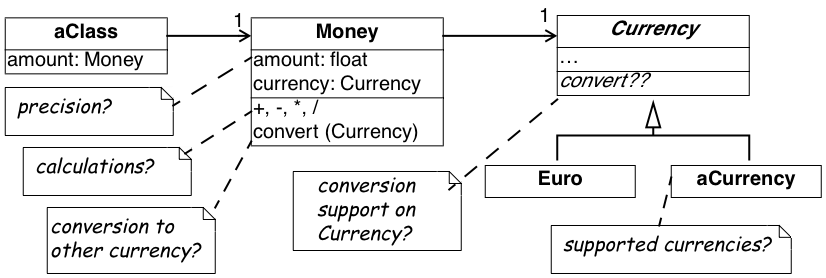
\includegraphics[width=\textwidth]{InitialCurrenciesA}
{\small (b) Refined hypothesis after verification against the source code; the 
modifications are shown as Notes}
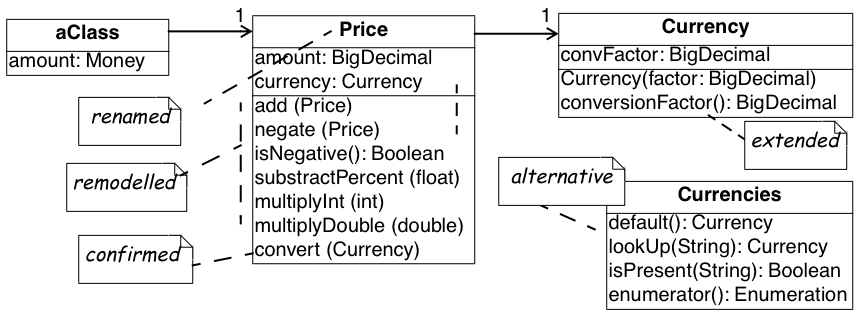
\includegraphics[width=\textwidth]{InitialCurrenciesB}
\caption{Refining the hypotheses concerning the Euro representation. (a) subclasses for the 
different currencies; (b) flyweight approach for the currencies}
\figlabel{InitialCurrencies}
\end{center}
\end{figure}

From a previous code review, you learned that the design is reasonably good, so you suspect 
that the designers have applied some variant of the \patpgref{Quantity}{Quantity} pattern. 
Therefore, you define an initial hypothesis in the form of the class diagram depicted in 
\figref{InitialCurrencies} (a). There is one class \lct{Money} holding two attributes; one 
for the amount of money (a floating point number) and one for the currency being used (an 
instance of the \lct{Currency} class). You assume operations on the \lct{Money} class to 
perform the standard calculations like addition, substraction, multiplication, $\cdots$ 
plus one operation for converting to another currency. \lct{Currency} should have 
subclasses for every currency supported and then operations to support the conversion from 
one currency into another. Of course, some questions are left unanswered and you note them 
down on your class diagram.

\begin{enumerate}
  \item What is the precision for an amount of \lct{Money}?

  \item Which calculations are allowed on an instance of \lct{Money}?

  \item How do you convert an instance of \lct{Money} into another currency?

  \item How is this conversion done internally? How is the support from the \lct{Currency} 
class?

  \item Which are the currencies supported?

\end{enumerate}

To answer these questions you verify your hypothesis against the source code and you adapt 
your class diagram accordingly. A quick glance at the filenames reveals a class 
\lct{Currency} but no class named \lct{Money}; a grep-search on all of the source code 
confirms that no class \lct{Money} exists. Browsing which packages import \lct{Currency}, 
you quickly find out that the actual name in the source code is \lct{Price} and you rename 
the \lct{Money} class accordingly.

Looking inside the \lct{Price} class reveals that the amount of money is represented as a 
fixed point number. There is a little comment-line stating:

\begin{code}
Michael (Oct 1999) -- Bug Report #324 -- Replaced
Float by BigDecimal due to rounding errors in the
floating point representation. Trimmed down the
permitted calculation operations as well.
\end{code}

Checking the interface of the \lct{Price} class you see that the calculation operations are 
indeed quite minimal. Only addition and negation (apparently substraction must be done via 
an addition with a negated operand) and some extra operations to take percentages and 
multiply with other numbers. However, you also spot a convert operation which confirms your 
hypothesis concerning the conversion of prices.

Next you look for subclasses of \lct{Currency}, but you don't seem to find any. Puzzled, 
you start thinking about alternative solutions and after a while you consider the 
possibility of a \patpgref{Flyweight}{Flyweight}. After all, having a separate subclass for 
each currency is a bit of an overhead because no extra behavior is involved. Moreover, with 
the flyweight approach you can save a lot of memory by representing all occurrences of the 
Euro-currency with a single Euro-object. To verify this alternative, you look for all 
occurrences of constructor methods for \lct{Currency} --- a \lct{grep Currency} does the 
trick --- and you actually discover a class \lct{Currencies} which encapsulates a global 
table containing all currencies accepted. Looking at the initialize method, you learn that 
the actual table contains entries for two currencies: Euro and Belgian Francs.

Finally, you study the actual conversion in a bit more detail by looking at the 
\lct{Price.convert} operation and the contents of the \lct{Currency} class. After some 
browsing, you discover that each \lct{Currency} has a single conversion factor. This makes 
you wonder: isn't conversion supposed to work in two ways and between all possible 
currencies? But then you check all invocations of the conversionFactor method and you 
deduce that the conversion is designed around the notion of a default currency (\ie the 
\lct{Currencies.default()} operation) and that the \lct{conversionFactor} is the one that 
converts the given currency to the default one. Checking the \lct{Price.convert operation}, 
you see that there is indeed a test for default currency in which case the conversion 
corresponds to a simple multiplication. In the other case, the conversion is done via a two 
step calculation involving an intermediate conversion to the default currency.

You're quite happy with your findings and you adapt your class diagram to the one depicted 
in figure 10(b). That model is annotated with the modifications you made to the original 
hypothesis, thus you store both the original and refined model into the configuration 
management system so that your colleagues can reconstruct your deduction process. You also 
file the following report summarizing your findings.

\noindent
\emph{Conversion to Euro.}
Facilities for Euro conversion are available, but extra work is required. One central class 
(Currencies) maintains a list of supported currencies including one default currency 
(Currencies.default). To convert to Euro, the initialization of this class must be changed 
so that the default becomes Euro. All prices stored in the database must also be converted, 
but this is outside the scope of my study.

Follow-up actions:

\begin{bulletlist}
\item Adapt initialization of class Currencies so that it reads the default currency and 
conversion factors from the configuration file.

\item Check the database to see how \lct{Prices} should be converted.
\end{bulletlist}

\subsection*{Rationale}

\begin{figure}
\begin{center}
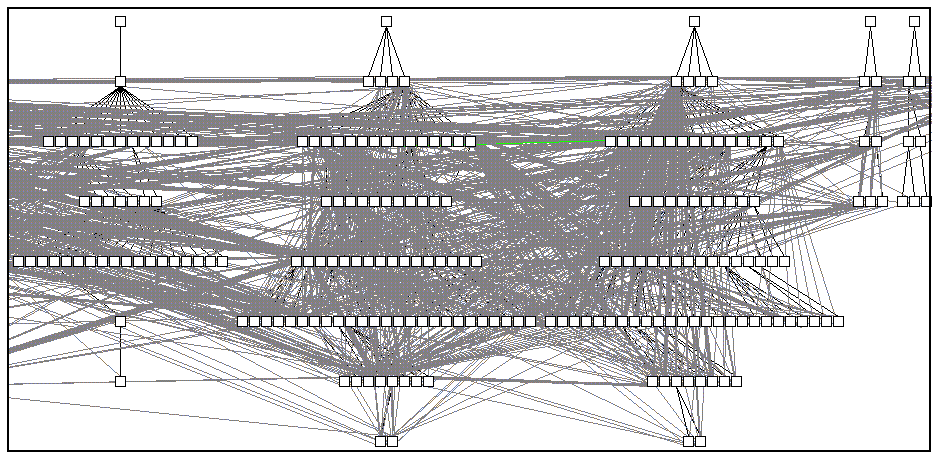
\includegraphics[width=\textwidth]{InitialWhiteNoise}
\caption{White-noise obtained by a bottom-up design extraction approach. The figure shows a 
fragment of an inheritance hierarchy augmented with all method invocations and attribute 
accesses for a medium sized system. The visualization is performed by \ind{CodeCrawler} 
\cite{Deme99c} \cite{Lanz99a}.}
\figlabel{InitialWhiteNoise}
\end{center}
\end{figure}

The naive approach to design extraction is bottom-up: first build a complete class diagram 
from source code and afterwards condense it by removing the noise. Unfortunately, the 
bottom-up approach does not work for large scale systems, because one typically gets a lot 
of white noise to start from (see for example \figref{InitialWhiteNoise}, showing an 
inheritance hierarchy with associations for a medium-sized system). Moreover, such a 
bottom-up approach does not improve your understanding very much, because it forces you to 
focus on the irrelevant noise instead of the important concepts.

\index{Cockburn, Alistair}
\begin{quotation}
\noindent
\emph{``We get things wrong before we get things right.''}

\hfill --- Alistair Cockburn, \cite{Cock93a}
\end{quotation}

In order to gain a true understanding of the legacy problem, you must go through a learning 
process. \patref{Speculate about Design}{SpeculateAboutDesign} is intended to stimulate 
such a learning process and therefore evidence that contradicts your hypothesis is as 
valuable as evidence that confirms it. Indeed, mismatches force you to consider alternative 
solutions and assess their pros and cons, and that is the moment when true understanding 
emerges.

\subsection*{Known Uses}

In \cite{Murp97a}, there is a report of an experiment where a software engineer at 
Microsoft applied this pattern (it is called ``the Reflection Model'' in the paper) to 
reverse engineer the C-code of Microsoft Excel. One of the nice sides of the story is that 
the software engineer was a newcomer to that part of the system and that his colleagues 
could not spend too much time to explain it to him. Yet, after a brief discussion he could 
come up with an initial hypothesis and then use the source code to gradually refine his 
understanding. Note that the paper also includes a description of a lightweight tool to 
help specifying the model, the mapping from the model to the source code and the checking 
of the code against the model.

The articles \cite{Bigg89c} \cite{Bigg93a} \cite{Bigg94a}, report several successful uses 
of this pattern (there it is called the ``concept assignment problem''). In particular, the 
authors describe a tool-prototype named \ind{DESIRE}, which includes advanced browsing 
facilities, program slicing and a Prolog-based query language. The tool has been used by a 
number of people in different companies to analyze programs of up to 220 KLOC. Other well-
known applications are reported by the \ind{Rigi} group, which among others have applied 
this pattern on a system consisting of over 2 million lines of PL/AS code \cite{Wong95a}.

It has been shown that such an approach can be used to map an object-oriented design onto a 
procedural implementation purely based on a static analysis of the source-code 
\cite{Gall99a} \cite{Weid98a}. Nevertheless, newer approaches try to exploit richer and 
more diverse information sources. \ind{DALI} for instance also analyses information from 
makefiles and profilers \cite{Bass98a} \cite{Kazm98b} \cite{Kazm99a}. Gaudi on the other 
hand, verifies the hypothesis against a mixture of the static call graphs with run-time 
traces \cite{Rich99a}.

\subsection*{What Next}

After this pattern, you will have a \subind{UML}{class diagram} representing a part of the 
design. You may want to \patref{Study the Exceptional Entities}
{StudyTheExceptionalEntities} to get an impression of the design quality. If you need a 
more refined model, consider the patterns in \chapgref{Detailed Model Capture}
{DetailedModelCapture}. When your reverse engineering efforts are part of a migration or 
reengineer project, you should cast your understanding of design in a test suite as 
explained in \chapgref{Tests: Your Life Insurance!}{TestsYourLifeInsurance}

%=================================================================
%:PATTERN -- {Study the Exceptional Entities}
\pattern{Study the Exceptional Entities}{StudyTheExceptionalEntities}

\intent{Identify potential design problems by collecting measurements and studying the 
exceptional values.}

\subsection*{Problem}

How can you quickly identify potential design problems in large software systems?

\emph{This problem is difficult because:}

\begin{bulletlist}
\item There is no easy way to discern problematic from good designs. Assessing the quality 
of a design must be done in the terms of the problem it tries to solve, thus can never be 
inferred from the design alone.

\item To confirm that a piece of code represents a design problem, you must first unravel 
its inner structure. With problematic code this is typically quite difficult.

\item The system is large, thus a detailed assessment of the design quality of every piece 
of code is not feasible.
\end{bulletlist}

\emph{Yet, solving this problem is feasible because:}

\begin{bulletlist}
\item You have a \emph{\ind{metrics} tool} at your disposal, so you can quickly collect a 
number of measurements about the entities in the source-code.

\item You have a \emph{rough understanding} of the system's functionality (for example 
obtained via \charef{First Contact}{FirstContact}), so you can assess the quality of the 
design in the system context.

\item You have the necessary \emph{tools to browse} the source-code, so you can verify 
manually whether certain entities are indeed a problem.
\end{bulletlist}

\subsection*{Solution}

Measure the structural entities forming the software system (\ie the inheritance hierarchy, 
the packages, the classes and the methods) and look for exceptions in the quantitative data 
you collected. Verify manually whether these anomalies represent design problems.

\subsubsection*{Hints}

Identifying problematic designs in a software system via measurements is a delicate 
activity which requires expertise in both data collection and interpretation. Below are 
some hints you might consider to get the best out of the raw numbers.

\begin{bulletlist}
\item \emph{Which tool to use?}
There are many tools --- commercial as well as public domain --- which measure various 
attributes of source code entities. Nevertheless, few development teams make regular use of 
such tools and therefore it is likely that you will have to look for a metrics tool before 
applying this pattern.

In principle, start by looking at the tools used by the development team and see whether 
they can be used to collect data about the code. For instance, a code verification tool 
such as lint can serve as basis for your measurements. Start looking for a metrics tool 
only when none of the development tools currently in use may collect data for you. If 
that's the case, simplicity should be your main tool adoption criterion as you do not want 
to spend your precious time on installing and learning. The second tool adoption criterion 
is how easy the metrics tool integrates with the other development tools in use.

\item \emph{Which metrics to collect?}
In general, it is better to stick to the simple metrics, as the more complex ones involve 
more computation, yet will rarely perform better.

For instance, to identify large methods it is sufficient to count the lines of code by 
counting all carriage returns or new-lines. Most other method size metrics require some 
form of parsing and this effort is usually not worth the gain.

\item \emph{Which metric variants to use?}
Usually, it does not make a lot of difference which metric variant is chosen, as long as 
the choice is clearly stated and applied consistently. Here as well, it is preferable to 
choose the most simple variant, unless you have a good reason to do otherwise.

For instance, while counting the lines of code, you should decide whether to include or 
exclude comment lines, or whether you count the lines after the source code has been 
normalized via pretty printing. However, when looking for potential design problems it 
usually does not pay off to do the extra effort of excluding comment lines or normalizing 
the source code.

\item \emph{Which thresholds to apply?}
Due to the need for reliability, it is better \emph{not} to apply thresholds.\footnote{Most 
metric tools allow you to focus on special entities by specifying some threshold interval 
and then only displaying those entities where the measurements fall into that interval.} 
First of all, because selecting threshold values must be done based on the coding standards 
applied in the development team and these you do not necessarily have access to. Second, 
thresholds will distort your perspective on the anomalies inside the system as you will not 
know how many normal entities there are.

%:HERE

\item \emph{How to interpret the results?}
An anomaly is not necessarily problematic, so care must be taken when interpreting the 
measurement data. To assess whether an entity is indeed problematic, it is a good idea to 
simultaneously inspect different measurements for the same entity. For instance, do not 
limit yourself to the study of large classes, but combine the size of the class with the 
number of subclasses and the number of superclasses, because this says something about 
where the class is located in the class hierarchy.

However, formulas that combine different measurements in a single number should be avoided 
as you loose the sense for the constituting elements. Therefore it is better to present the 
results in a table, where the first column shows the name of the entity, and the remaining 
columns show the different measurement data. Sorting these tables according to the 
different measurement columns will help you to identify exceptional values.

\item \emph{How to identify anomalies quickly?}
Although it is possible to identify exceptional values in a tabular representations of 
measurement data, such an approach is tedious and error-prone. Most metric tools include 
some visualization features (histograms, scatter plots, $\cdots$) to help you scan large 
volumes of measurements and this is usually a better way to quickly focus on potential 
design problems.

\item \emph{Should I browse the code afterwards?}
Measurements alone cannot determine whether a entity is truly problematic: some human 
assessment is always necessary. Metrics are a great aid in quickly identifying entities 
that are potential problems but code browsing is necessary for confirmation. Note that 
large entities are usually quite complicated, thus understanding the corresponding source 
code may prove to be difficult.

\item \emph{What about normal entities?}
Experienced programmers tend to distribute important functionality over a number of well-
designed components. Conversely, exceptional entities are quite often irrelevant as truly 
important code would have been refactored. Therefore, you should be aware that you are only 
applying a heuristic: its possible that you are studying code which does not represent a 
design problem simply because it is deemed unimportant.
\end{bulletlist}

\subsection*{Tradeoffs}

\subsubsection*{Pros}

\begin{bulletlist}
\item \emph{Scales well.}
Metrics are readily applicable to large scale systems, mainly because with metric tools 
about 20\% of all the entities require further investigation. When different metrics are 
combined properly (preferably using some form of visualization) one can deduce quite 
rapidly which parts of the system represent potential design problems.

\item \emph{Overview mode is appealing.}
With proper tool support you can produce visual representations of the metrics data that 
provide immediate insight into the good as well as the problematic parts of the design.
\end{bulletlist}

\subsubsection*{Cons}

\begin{bulletlist}
\item \emph{Results are inaccurate.}
Some of the entities having exceptional measurements will turn out not to be problematic. 
Metrics are only a heuristic and false positives are likely to occur. Moreover, the metric 
may reveal problems that are not worth solving because the solutions will not contribute to 
your reengineering goal. Unfortunately, this you will only know after you analyzed the 
source code.

\item \emph{Missing priorities.}
Identifying a potential problem is easy, the real difficult part is assessing the severity 
of the problem. Especially during a reengineering project, you identify far more problems 
than you have time to solve. Prioritizing the list requires a good understanding of both 
the system and the reengineering project.
\end{bulletlist}

\subsubsection*{Difficulties}

\begin{bulletlist}
\item \emph{Data is tedious to interpret.} To measure the quality of a piece of code, you 
must collect several measurements. Interpreting and comparing such multi-valued tuples is 
quite tedious especially when dealing with large software systems. Therefore, use 
visualizations which allow you to analyze different measurements simultaneously.

\item \emph{Requires expertise.}
The interpretation of measurement data is difficult and requires a lot of expertise. 
Fortunately, part of this expertise is documented in the form of design heuristics (see 
among others \cite{Riel96a} \cite{Lore94a}) and the rest can be acquired on the job.
\end{bulletlist}

\subsection*{Example}

The analysis of the database and the design of \emph{XDoctor} was quite reassuring. 
Although there were some things to improve, the overall quality was quite good. Yet, you 
want to confirm this feeling and therefore plan to collect a number of quality metrics and 
visualize them. (Of course the visualization can be done with ordinary spreadsheets, but in 
this case you decide to use the CodeCrawler tool \cite{Deme99c} \cite{Lanz99a}.)

\begin{figure}
\begin{center}
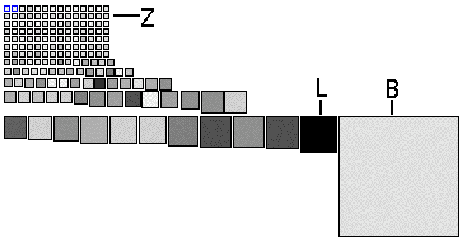
\includegraphics[width=0.6\textwidth]{InitialClassSize}
\caption{Class size overview with node size showing the lines of code and gray value 
showing the number of instance variables.}
\figlabel{InitialClassSize}
\end{center}
\end{figure}

\noindent
\emph{Class Size Overview.}
As a starter, you get an impression of the raw physical size of all the classes 
constituting \emph{XDoctor}. You measure the class size in terms of number of lines of code 
(LOC) and number of instance variables (NIV) and use a \emph{checkers graph} to show the 
relative proportion of the sizes. In such a graph all nodes are shown as squares where the 
size of the square is proportional to one size (here LOC) and the gray value is 
proportional to another size (here NIV).

\figref{InitialClassSize} shows the checker graph for \emph{XDoctor}. The picture reveals 
that the class size is distributed quite evenly --- which is reassuring --- with a few 
noteworthy exceptions. For instance, there is the class B (with 1495 it is the largest in 
terms of lines of code) and class L (has most instance variables and second most lines of 
code). The classes in row Z are exceptional in the sense that they are very small, some of 
them even empty.

\noindent
\emph{Class Inheritance.}
Next, you get a feeling for the way inheritance is used by studying the various subtrees in 
the inheritance hierarchy. Therefore, you measure the classes in terms of hierarchy nesting 
level (HNL) and number of descendant classes (NDC). You include size measurements as well 
to assess the magnitude of the classes within the inheritance tree. Therefore, you collect 
the number of methods (NOM), number of instance variables (NIV) and number of lines of code 
(LOC) as well. You use an \emph{inheritance tree} to visualize the various subtrees and the 
proportion of class sizes inside each of them. All nodes in such a tree have a rectangular 
shape where the height, width and gray value of each node show three measurements.

\begin{figure}
\begin{center}
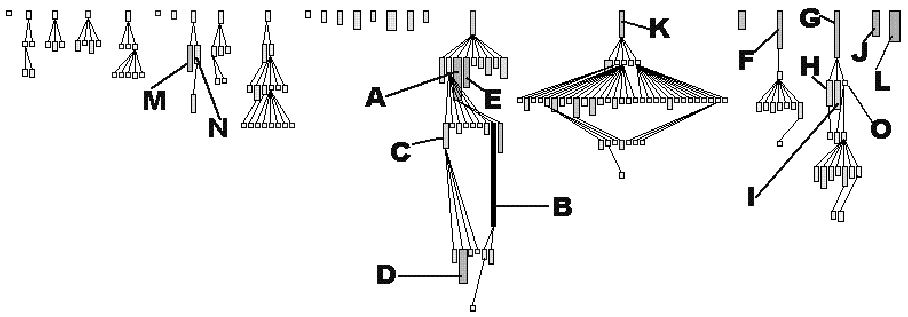
\includegraphics[width=\textwidth]{InitialInheritanceTree}
\caption{Inheritance tree focussing on class size. The node width shows the number of 
instance variables, the node height shows the number of methods and the gray value shows 
the number of code lines.}
\figlabel{InitialInheritanceTree}
\end{center}
\end{figure}

\figref{InitialInheritanceTree} shows such an inheritance tree for \emph{XDoctor}, where 
the height, width and gray value of each node represent NOM, NIV and LOC. To the left, you 
observe several normal inheritance trees, namely small ones where the size of the classes 
is quite similar. One exceptional value is the same B you noticed earlier, however you now 
see that it also has a large superclass A (defining 70 methods), making it even more 
suspicious. The L you've seen before appears here as a solitary class. The hierarchies 
rooted in K, F and G seem quite interesting: they go deep (4 levels of inheritance) and 
have one large root class plus many smaller subclasses. H and I, plus M and N are both 
cases of large sibling classes, which may imply that too little is inherited from the 
common superclass. This must be verified via code browsing however.

\noindent
\emph{Method Inheritance.}
To analyze particular inheritance trees in further detail, you investigate how methods in a 
subclass relate to methods in their superclass. Therefore, you produce a table showing for 
each class the number of methods overriding a method defined in a superclass (NMO), the 
number of methods added to the superclass (NMA) and the number of methods extending a 
method defined in a superclass (NME). Here as well you use an inheritance tree to identify 
exceptional values in the measurements.

\begin{figure}
\begin{center}
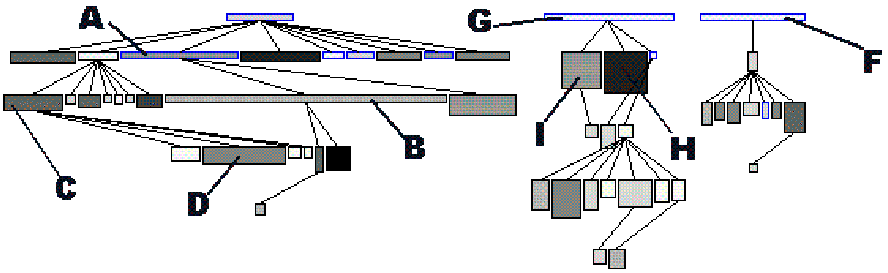
\includegraphics[width=\textwidth]{InitialMethodInheritance}
\caption{Inheritance tree focussing on method inheritance. The node width shows the number 
of methods added, the node height shows the number of methods overridden and the gray value 
shows the number of methods extended.}
\figlabel{InitialMethodInheritance}
\end{center}
\end{figure}

\figref{InitialMethodInheritance} shows the A, G and F subtrees identified earlier, but now 
the height, width and gray value of each node represent NMO, NMA and NME. The root classes 
are displayed as narrow white rectangles, which is normal as root classes cannot override 
nor extend. As far as the subclasses concerns, you observe two phenomena. On the one hand, 
the subclasses of A add a lot, yet override very little, which suggests that code reuse is 
the main purpose of this inheritance tree. On the other hand, the subclasses of F and G 
override more methods than they add, which suggests a lot of hook methods and an 
inheritance tree aimed at specializing behavior. Here as well, these assumptions must be 
verified by code browsing. 

\noindent
\emph{Method Size Overview.}
An example of how to identify potential problems in the method bodies concerns the ratio of 
lines of code (LOC) and the number of messages sent (MSG). In most method bodies, these two 
measurements will correlate but methods where this correlation does not hold typically 
represent special code.

To study this correlation relationship one might divide the two measurements.
\footnote{Metrics theory prohibits arbitrary manipulations of numbers; one should Þrst 
verify whether the scale of the measurement permits the calculation \cite{Fent96a}. 
However, both are counting measurements having a ratio scale and then division is 
permitted.} However, then you lose the sense for the constituting measurements which makes 
interpretation difficult. Therefore, you visualize the relationship by means of a 
\emph{correlation graph}, where each method is shown as a small square and where the x, y 
position shows the measurements that are supposed to correlate. In such a graph, the nodes 
where the measurements correlate cluster around a diagonal, while the exceptions are from 
the diagonal.

\begin{figure}
\begin{center}
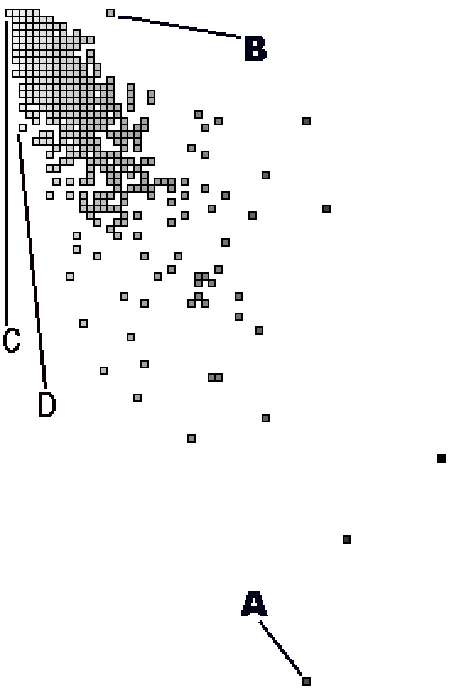
\includegraphics[width=0.4\textwidth]{InitialCorrelationGraph}
\caption{Correlation graph, with x-position showing the number of messages 
sent and y-position showing the lines of code.}
\figlabel{InitialCorrelationGraph}
\end{center}
\end{figure}

\figref{InitialCorrelationGraph} shows a correlation graph where the horizontal axis (left 
to right) represents the number of messages sent and the vertical axis (top to bottom) the 
number of lines of code. You observe a big cluster in the top left corner where most nodes 
are superimposed on each other. This is reassuring because it implies that most methods 
have fewer than 15 lines of code and 10 messages sent. The exceptions appear at the edges 
of the picture. For instance, node A is a large method with 99 messages packed on 45 lines 
of code. Node D (and its neighbors) are also methods where many messages are packed on a 
single line of code. Via code browsing you see that many of them are initialization 
methods. At the other side of the diagonal there is node B, which represents a method with 
16 lines of code yet no messages sent. Code browsing reveals that it's a case where the 
whole method body has been commented out.

\subsection*{Rationale}

\index{De Marco, Tom}
\begin{quotation}
\noindent
\emph{You cannot control what you cannot measure.}

\hfill --- Tom De Marco, \cite{Dema82a}	 
\end{quotation}

In several places in the literature it is mentioned that measuring source code helps in 
problem identification (see among others, \cite{Lore94a} \cite{Fent96a} \cite{Mayr96a} 
\cite{Nesi98a}). Most metric tools applied during these experiments visualize information 
by means of histograms and Kiviat diagrams. However, few research have studied the impact 
of thresholds while identifying exceptional entities; our own experience is that thresholds 
don't really matter \cite{Deme99a}.

Unfortunately, the current research is inconclusive with regards to the accuracy of the 
results. Up until now, no experiments exist that count how many problems remain 
undiscovered, nor is there any work on assessing the severity of the problems discovered. 
As such it is impossible to assess the reliability of metrics for reverse engineering.

\subsection*{Known Uses}

During the \ind{FAMOOS} project one event provided anecdotal evidence for how well a simple 
approach may outperform more specialized and complex approaches. Once we visited a business 
unit for a few days to demonstrate our \ind{CodeCrawler} tool. At first the developers were 
quite sceptical because they felt like they would see ``yet another metrics tool''. The 
first surprise came when we showed them results already during the first day. They told us 
that other tools would typically require several days configuration time before they could 
parse their C++ code because it made such heavy use of special C++ features and macros. 
Moreover, and this was the second surprise, this simplicity did not diminish the quality of 
our results. The programmers confirmed most of the design anomalies we discovered, yet were 
intrigued by some observations we made. During the subsequent discussions they at least 
considered design alternatives.

\subsection*{What Next}

Applying this pattern will result in an overall impression of design quality and the 
identification of a few potential design problems. With this knowledge you should at least 
reconsider whether the goal of your reengineering project is still attainable. If it is, 
you will probably want to solve some of these design problems, for instance using patterns 
in \chapgref{Redistribute Responsibilities}{RedistributeResponsibilities} and 
\chapgref{Transform Conditionals to Polymorphism}{TransformConditionalsToPolymorphism}. 
Solving some of these problems may require a more detailed understanding of that design, 
which may be obtained by patterns in \chapgref{Detailed Model Capture}
{DetailedModelCapture}.

%=============================================================
\ifx\wholebook\relax\else
   \bibliographystyle{alpha}
   \bibliography{scg}
   \end{document}
\fi
%=============================================================
